\chapter{Desenvolvimento}

A partir do desenvolvimento de uma aplicação, que pode ser embarcada em um hardware modesto e utilizada com conexões precárias, em conjunto de diversos tipos de sensores visa-se atender este mercado de monitoramento e controle de ambientes. Assim, tratar-se-á, neste capítulo, sobre o desenvolvimento do projeto de cliente e servidor CoAP, em que é possível visualizar a implementação exposta no diagrama abaixo.

\begin{figure}[!htb]
	\centering
	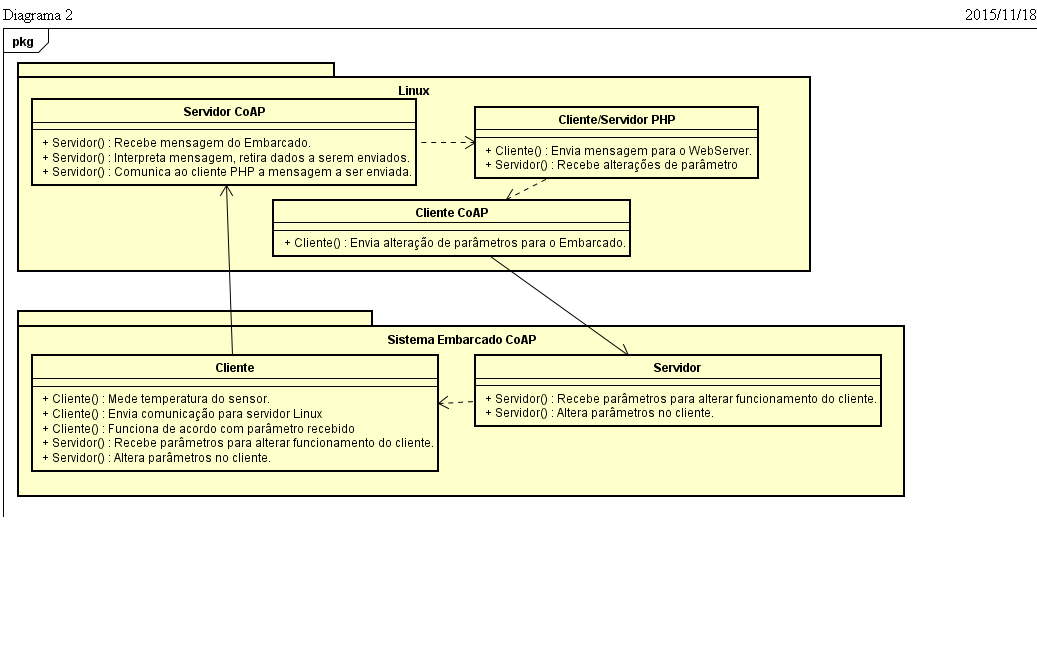
\includegraphics[width=1.0\textwidth]{../Diagrama_sem_webserver.png}
	\caption{Diagrama 1}
	\label{fig:Diagrama_lin_emb}
\end{figure}



Ainda que demonstrado cliente e servidor juntos, este projeto foi pensado e desenvolvido para ser utilizado de forma separada também. A implementação de ambos os elementos será descrita individualmente, e, por fim, será descrito o funcionamento delas em conjunto.

\section{Cliente CoAP}
O cliente foi desenvolvido em C, visando a aumentar a possibilidade de implantação em embarcados de baixo custo e melhoria de performance. A mensagem será transportada pelo protocolo UDP, utilizando o protocolo de aplicação CoAP. O funcionamento será dividido e descrito nas próximas seções, para melhor entendimento.


\subsection{Conexão}
Como visto, utilizaremos o protocolo UDP para transporte, então faremos a conexão, como demonstrada abaixo:

\begin{lstlisting}
//CONEXAO
int fd;

struct sockaddr_in servaddr;
fd = socket(AF_INET,SOCK_DGRAM,0);
bzero(&servaddr,sizeof(servaddr));
servaddr.sin_family = AF_INET;
servaddr.sin_addr.s_addr = inet_addr("192.168.1.20");
servaddr.sin_port = htons(7891);
bind(fd,(struct sockaddr *)&servaddr, sizeof(servaddr));
\end{lstlisting}

Ligando o socket a porta e endereço do servidor, via UDP.
O envio da mensagem é feito da seguinte forma:

\begin{lstlisting}
if (rand()%100<PORCENTAGEM)
{
printf("\n\nSending\n\n");
sendto(fd, buf_out, rsplen, 0, (struct sockaddr *) &cliaddr, sizeof(cliaddr));
}
else
{
printf("\n\nNot sending, simulando erro de comunicação\n\n");
}    
\end{lstlisting}

Foi utilizada a função \texttt{if(rand()\%100<PORCENTAGEM)} para simular a perda de pacotes em conexões limitadas.


\subsection{Criação do pacote}

Foi usada a função \texttt{cria\_pkt } , e essa, por sua vez, chama a função \texttt{monta\_header\_token }, para criação do \textit{header} e \textit{token} do pacote, que são pré-definidos, no caso de o \textit{token} utilizado ser gerado pelo programa e não pelo usuário. 

\begin{lstlisting}
void monta_header_token (coap_packet_t *pkt, uint8_t *token)
{
	pkt->hdr.ver = 	 0x01; // versão 01;
	pkt->hdr.t = 	 0x00; // code 0 (confirmable);
	pkt->hdr.code =  0x02; //request -> 0000 0010 -> POST, 0000 0011 -> PUT
	srand(time(NULL));
	short int var_aux = rand()%254;
	pkt->hdr.id [0] = var_aux;
	short int var_aux = rand()%254;
	pkt->hdr.id [1] = var_aux;
	pkt->tok.p = token;
	pkt->tok.len = strlen(token);
	pkt->hdr.tkl = pkt->tok.len;
}
\end{lstlisting}

Foram empregadas as funções \texttt{srand, rand()} para gerar aleatoriamente valores para o \textit{id} e para o \textit{token}, que foi gerado de forma similar a utilizada para gerar o \textit{id}, porém não foi transposta para o trecho acima. 

\subsection{Parâmetros}

Inicialmente foi pensado em receber os parâmetros via linha de comando, passando-os como argumentos para a função.
Porém, além de dificultar os testes, posterior a criação do cliente, foi pensado em fazer do cliente uma função do servidor. Para isso, uma mensagem padrão foi criada, com \textit{options} definidas e necessitando alterar apenas o payload, com \textit{token} gerado de forma aleatória.
Como a função de identificação e verificação de parâmetros já havia sido feita para receber os parâmetros via linha de comando, apenas foi necessária uma adaptação da mensagem, para se encaixar nos moldes utilizados pela função padrão de recebimento de parâmetros, assim, a função seguinte de identificação não faz distinção entre o método empregado para envio de parâmetros utilizado.
A função utilizada para este fim, de alterar a mensagem pré-pronta deixando-a nos moldes da versão anterior, foi a \texttt{separa_string}.

\subsection{Verificação e interpretação dos argumentos}

Aqui utilizaremos parte da função \texttt{identifica\_arg} para explicar como foi feita a identificação dos argumentos.
\begin{lstlisting}
void identifica_arg (coap_packet_t *pkt, int argc, char **argv, char *buf_aux_opt_c, short int *buf_aux_opt_n)
{
	...
	else if(strcmp(argv[j], "-op") == 0)
	{
		if (j+3 > argc) //caso não tenha os campos necessários
		{
			lida_erro_id(erro_argumento_num_option_invalido, argc, argv);
		}
		else if(veri_option (argv[j+1], argv[j+2]))
		{
			lida_erro_id(erro_argumento_num_option_invalido, argc, argv);
		}
		else
		{
			add_option(pkt, cont_aux, &buf_aux_opt_n[cont_op-1], argv[j+2], cont_op, &option_delta);
			j+=3;
		}
	}
	...
}
\end{lstlisting}

Como podemos ver, é feita uma verificação dos parâmetros, verificando se são argumentos válidos , com a função \texttt{veri\_option()} e caso sejam, adicionando ao pacote criado. A seguir será descrita com mais detalhes as funções \texttt{add_token}, \texttt{add_option} e \texttt{add_payload}. 

\subsubsection{Funções de adicionar payload, option, token}
Este é um tipo de subseção

\subsection{Monta pacote}
Como visto no diagrama, a mensagem é montada no pacote (\texttt{&pkt}) e enviada através do buffer de saída (\texttt{buf_out}). Essa tarefa é feita pela função \texttt{monta_pkt}.




\subsection{Buffer}
Este é um tipo de subseção

\subsection{Separação de palavras}
Este é um tipo de subseção

\subsection{Lidar mensagem}
Este é um tipo de subseção

\subsubsection{Subsubseção1}
Este tipo de subsubsection

%\paragraph{Seção quinária}
Este é um tipo de seção quinária

